\documentclass[letterpaper,10pt]{article}

\usepackage{enumitem}
\usepackage{titling}
\usepackage{listings,listings-rust}
\usepackage{url}
\usepackage{soul}
\usepackage{hyperref}
\usepackage{setspace}
\usepackage{subfig}
\usepackage{sectsty}
\usepackage{pdfpages}
\usepackage{colortbl}
\usepackage{multirow}
\usepackage{multicol}
\usepackage{relsize}
\usepackage{amsmath}
\usepackage{wasysym}
\usepackage{fancyvrb}
\usepackage[yyyymmdd]{datetime}
\usepackage{amsmath,amssymb,amsthm,graphicx,xspace}
\usepackage[titlenotnumbered,noend,noline]{algorithm2e}
\usepackage[compact]{titlesec}
\usepackage{XCharter}
\usepackage[T1]{fontenc}
\usepackage[scaled]{beramono}
\usepackage[normalem]{ulem}
\usepackage{booktabs}
\usepackage{tikz}
\usetikzlibrary{arrows.meta,automata,shapes,trees,matrix,chains,scopes,positioning,calc,decorations.pathreplacing}
\tikzstyle{block} = [rectangle, draw, fill=blue!20, 
    text width=2.5em, text centered, rounded corners, minimum height=2em]
\tikzstyle{bw} = [rectangle, draw, fill=blue!20, 
    text width=4em, text centered, rounded corners, minimum height=2em]

\definecolor{namerow}{cmyk}{.40,.40,.40,.40}
\definecolor{namecol}{cmyk}{.40,.40,.40,.40}
\renewcommand{\dateseparator}{-}

\let\LaTeXtitle\title
\renewcommand{\title}[1]{\LaTeXtitle{\textsf{#1}}}

\lstset{basicstyle=\footnotesize\ttfamily,breaklines=true}

\newcommand{\CPP}{C\nolinebreak\hspace{-.05em}\raisebox{.4ex}{\tiny\bf +}\nolinebreak\hspace{-.10em}\raisebox{.4ex}{\tiny\bf +}}
\def\CPP{{C\nolinebreak[4]\hspace{-.05em}\raisebox{.4ex}{\tiny\bf ++}}}

\newcommand{\handout}[5]{
  \noindent
  \begin{center}
  \framebox{
    \vbox{
      \hbox to 5.78in { {\bf ECE459: Programming for Performance } \hfill #2 }
      \vspace{4mm}
      \hbox to 5.78in { {\Large \hfill #4  \hfill} }
      \vspace{2mm}
      \hbox to 5.78in { {\em #3 \hfill \today} }
    }
  }
  \end{center}
  \vspace*{4mm}
}

\newcommand{\lecture}[3]{\handout{#1}{#2}{#3}{Lecture#1}}
\newcommand{\tuple}[1]{\ensuremath{\left\langle #1 \right\rangle}\xspace}

\addtolength{\oddsidemargin}{-1.000in}
\addtolength{\evensidemargin}{-0.500in}
\addtolength{\textwidth}{2.0in}
\addtolength{\topmargin}{-1.000in}
\addtolength{\textheight}{1.75in}
\addtolength{\parskip}{\baselineskip}
\setlength{\parindent}{0in}
\renewcommand{\baselinestretch}{1.5}
\newcommand{\term}{Winter 2020}

\singlespace


\begin{document}

\lecture{13 --- Dependencies and Speculation }{\term}{Patrick Lam and Jeff Zarnett}

\section*{Dependencies}
Some computations appear to be ``inherently sequential''. There are plenty of real-life analogies:

\begin{itemize}
\item must extract bicycle from garage before closing garage door
 
\item must close washing machine door before starting the cycle
 
\item must be called on before answering questions? (sort of, some people shout out...)
 
\item students must submit assignment before course staff can mark the assignment (also sort of... I can assign you a grade of zero if you didn't submit an assignment!)
\end{itemize}

There are some prerequisite steps that need to be taken before a given step can take place. The problem is that we need some result or state from an earlier step before we can go on to the next step. Interestingly, in many of the analogies, sometimes if you fail to respect the dependency, nothing physically stops the next step from taking place, but the outcome might not be what you want (\ldots you don't want zero on your assignment, right?).

The same with dependencies in computation. If you need the result of the last step you will have to wait for it to be available before you can go on to the next. And if you jump the gun and try to do it early, you will get the wrong result (if any at all). 

Note that, in this lecture, we are going to assume that we don't have data races. This reasoning is not guaranteed to work in the presence of undefined behaviour, which exists when you have data races.

\paragraph{Main Idea.} A \emph{dependency} prevents parallelization
when the computation $XY$ produces a different result from the
computation $YX$. That is to say, there is a correct order for doing these two steps and getting the order wrong means we get the wrong outcome. If you want to bake a cake, you have to mix all the ingredients before you bake them; if you bake all ingredients and then mix them, whatever you get isn't a cake.

Remember, of course, that there are lots of things that don't have dependencies and can be done in arbitrary order (or even concurrently). If your household chores are to vacuum the floor and do the laundry, you get a valid outcome no matter what order you do them in, as long as you do both correctly. The outcome is the same!

There are two kinds of dependency that we'll cover and they are \emph{loop-carried} and \emph{memory-carried} dependencies.

\paragraph{Loop-Carried Dependencies.} Let's start with the loop-carried version. In this kind of dependency, executing an iteration of the loop depends on the result of the previous iteration. Initially, {\tt vec[0]} and {\tt vec[1]} are 1. Can we run these lines in parallel?

\begin{lstlisting}[language=Rust]
let mut vec = vec![1; 32];
    /* */
vec[4] = vec[0] + 1;
vec[5] = vec[0] + 2;
\end{lstlisting}


It turns out that there are no dependencies between the two lines. But this is
an atypical use of arrays. Let's look at more typical uses.

What about this? (Again, all elements initially 1.)

\begin{lstlisting}[language=Rust]
for i in 1 .. vec.len() {
    vec[i] = vec[i-1] + 1;
}
\end{lstlisting}

Nope! We can unroll the first two iterations:
\begin{lstlisting}[language=Rust]
vec[1] = vec[0] + 1;
vec[2] = vec[1] + 1;
\end{lstlisting}

Depending on the execution order, either {\tt vec[2] = 3} or {\tt vec[2] =
  2}.  In fact, no out-of-order execution here is safe---statements depend
on previous loop iterations, which exemplifies the notion of a
\emph{loop-carried dependency}. 

Okay, that's perhaps a silly example. 
Let's try a real problem. Consider this code to compute whether a complex number $x_0 + iy_0$ belongs to the Mandelbrot set.

\begin{lstlisting}[language=Rust]
// Repeatedly square input, return number of iterations before
// absolute value exceeds 4, or 1000, whichever is smaller.
fn mandelbrot(x0: f64, y0: f64) -> i32 {
    let mut iterations = 0;
    let mut x = x0;
    let mut y = y0;
    let mut x_squared = x * x;
    let mut y_squared = y * y;
    while (x_squared + y_squared < 4f64) && (iterations < 1000) {
        y = 2f64 * x * y + y0;
        x = x_squared - y_squared + x0;
        x_squared = x * x;
        y_squared = y * y;
        iterations += 1;
    }
    return iterations;
}
\end{lstlisting}
In this case, it's impossible to parallelize loop iterations, because
each iteration \emph{depends} on the $(x, y)$ values calculated in the
previous iteration. For any particular $x_0 + iy_0$, you have to run the
loop iterations sequentially.

That doesn't mean that the problem cannot be parallelized at all, however.
You can parallelize the Mandelbrot set calculation
by computing the result simultaneously over many points at
once, even if each point's calculation needs to be done sequentially.
Indeed, that is a classic ``embarassingly parallel'' problem,
because the you can compute the result for all of the points
simultaneously, with no need to communicate.

 Now consider this example---is it parallelizable? (Again, all elements initially 1.)

\begin{lstlisting}[language=C]
for i in 4 .. vec.len() {
    vec[i] = vec[i-4] + 1;
}
\end{lstlisting}

Yes, to a degree. We can execute 4 statements in parallel at a time:
\begin{itemize}
  \item \texttt{vec[4] = vec[0] + 1, vec[8] = vec[4] + 1}
  \item \texttt{vec[5] = vec[1] + 1, vec[9] = vec[5] + 1}
  \item \texttt{vec[6] = vec[2] + 1, vec[10] = vec[6] + 1}
  \item \texttt{vec[7] = vec[3] + 1, vec[11] = vec[7] + 1}
\end{itemize}  
We can say that the array accesses have stride 4 --- there are no
dependencies between adjacent array elements. In general, consider
dependencies between iterations.


\paragraph{Memory-Carried Dependencies.} On the other hand, a memory-carried dependency is one where the result
of a computation \emph{depends} on the order in which two memory accesses
occur. For instance:

{\small \begin{lstlisting}[language=Rust]
let mut acct: Account = Account {
    balance: 0.0f32
};
f(&mut acct);
g(&mut acct);

/* */

fn f (a: &mut Account) {
    a.balance += 50.0f32;
}
fn g (a: &mut Account) {
    a.balance *= 1.01f32;
}
\end{lstlisting} }

{\sf What are the possible outcomes after executing {\tt g()} and {\tt f()}
in parallel threads? Obviously, assuming they are properly wrapped in Atomic reference counted types to allow the code to compile.} \\[1em]


\section*{Critical Paths}
You should be familiar with the concept of a critical path from other courses (e.g., capstone design project) or just from project management you've experienced on coop terms. 
It is the minimum amount of time to complete the task, taking dependencies into account.
Consider the following diagram, which illustrates dependencies between
tasks (shown on the arrows). 
Note that B depends on A, and D depends on B and C, but C does
not depend on anything, so it could be done in parallel with
everything else. You can also compute expected execution times
for different strategies.
\begin{center}
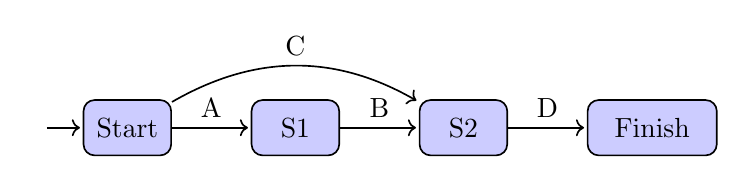
\begin{tikzpicture}[->,shorten >=1pt,auto,column sep=2.2cm,
                    semithick,initial text=]
  \node[initial,block] (s0) {Start};
  \node[block] (s1) [right=of s0] {S1};
  \node[block] (s2) [right=of s1] {S2};
  \node[bw] (s3) [right=of s2] {Finish};

  \path (s0) edge node {A} (s1)
        (s1) edge node {B} (s2)
        (s2) edge node {D} (s3)
        (s0) edge[bend left=30] node {C} (s2);
\end{tikzpicture}
\end{center}

 Having a diagram like this makes it easy to see what can run in parallel and what steps need to happen in what order.  You might not need such a thing, but they are super useful for explaining to nontechnical coworkers or senior management what is happening and how it's going.


\section*{Breaking Dependencies with Speculation}
Let's go back to a real life analogy of speculation. Under normal circumstances, the coffee shop staff waits for you to place your order (``medium double double'') before they start making your order. Sensible. If you go to a certain coffee shop enough, then the staff start to know you and know your typical order and they might speculate about your order and start preparing it in advance, even before you get up to the counter. If they're right, time is saved: your order is ready sooner. If they're wrong, the staff did some unnecessary work and they'll throw away that result and start again with what you did order. If they can predict with high accuracy what you will order, then this is a net savings of time on average.

You can even put some numbers on it! If successfully predicting your order saves 30 seconds per day, and if they're wrong, remaking it takes 3 minutes longer than normal, then if your order is unpredictable one out of every 10 days, how much time is saved? 9 days are correct for a savings of 4.5 minutes, from which we subtract the 3 minute penalty for being wrong, and we've saved 1.5 minutes in the 10 day period (or about 15 seconds per day on average). Not huge, but imagine if the coffee shop can do that for every regular customer. If there are 100 regular customers that's 25 minutes of waiting saved per day! It all adds up.

Mind you, the idea of speculation isn't new in this course.
Recall that computer architects often use speculation to predict branch
targets: the direction of the branch depends on the condition codes
when executing the branch code. To get around having to wait, the processor
speculatively executes one of the branch targets, and cleans up if it
has to.

We can also use speculation at a coarser-grained level and
speculatively parallelize code. We discuss two ways of doing so: one
which we'll call speculative execution, the other value speculation.

\paragraph{Speculative Execution for Threads.} The idea here is to
start up a thread to compute a result that you may or may not need.
Consider the following code:

\begin{lstlisting}[language=Rust]
fn do_work(x: i32, y: i32, threshold: i32) -> i32 {
    let val = long_calculation(x, y);
    if val > threshold {
        return val + second_long_calculation(x, y);
    }
    return val;
}
\end{lstlisting}
Without more information, you don't know whether you'll have to execute
{\tt second\_long\_calculation()} or not; it depends on the return value of
{\tt long\_calculation()}.  Fortunately, the arguments to {\tt second\_long\_calculation()} do not
depend on {\tt long\_calculation()}, so we can call it at any point. 
Here's one way to speculatively thread the work:

\begin{lstlisting}[language=Rust]
fn do_work(x: i32, y: i32, threshold: i32) -> i32 {
    let t1 = thread::spawn(move || {
        return long_calculation(x, y);
    });
    let t2 = thread::spawn(move || {
        return second_long_calculation(x, y);
    });
    let val = t1.join().unwrap();
    let v2 = t2.join().unwrap();
    if val > threshold {
        return val + v2;
    }
    return val;
}
\end{lstlisting}
We now execute both of the calculations in parallel and return the same
result as before. Is this the only way to do it? No. The current thread is a valid thread for doing work and we don't have to create two threads and join two threads: we can create one and maybe have less overhead.

\begin{lstlisting}[language=Rust]
fn do_work(x: i32, y: i32, threshold: i32) -> i32 {
    let t1 = thread::spawn(move || {
        return second_long_calculation(x, y);
    });
    let val = long_calculation(x, y);
    let v2 = t1.join().unwrap();
    if val > threshold {
        return val + v2;
    }
    return val;
}
\end{lstlisting}

{\sf Intuitively: when is this code faster? When is it slower? How
  could you improve the use of threads?}\\[4em]

We can model the above code by estimating the probability $p$ that
the second calculation needs to run, the time $T_1$ that it takes
to run {\tt long\_calculation}, the time $T_2$ that it takes to run
{\tt second\_long\_calculation}, and synchronization overhead $S$.
Then the original code takes time
\[ T = T_1 + p T_2, \]
while the speculative code takes time
\[ T_s = \max(T_1, T_2) + S.\]

\paragraph{Exercise.} Symbolically compute when it's profitable to do the
speculation as shown above. There are two cases: $T_1 > T_2$ and $T_1
< T_2$. (You can ignore $T_1 = T_2$.)


\paragraph{Value Speculation.}
The other kind of speculation is value speculation. In this case,
there is a (true) dependency between the result of a computation 
and its successor:
% note: v1 is meant to be the result you get from longCalculation this time, while last_value is what you got last time. (The code doesn't show that). If you get the same result from longCalculation this time as you did last time, then secondLongCalculation is correct and you don't need to redo it.

\begin{lstlisting}[language=Rust]
fn do_other_work(x: i32, y: i32) -> i32 {
    let val = long_calculation(x, y);
    return second_long_calculation(val);
}
\end{lstlisting}

If the result of {\tt value} is predictable, then we can speculatively
execute {\tt second\_long\_calculation} based on the predicted value.
(Most values in programs are indeed predictable). If 90\% of customers are using the standard billing plan, you might assume that that's correct in your calculations, and then change that later if it turns out you are wrong. Or you might have a software cache where you keep the latest state so you don't have to go to the database to check a value that changes rarely. 

\begin{lstlisting}[language=Rust]
fn do_other_work(x: i32, y: i32, last_value: i32) -> i32 {
    let t = thread::spawn(move || {
        return second_long_calculation(last_value);
    });
    let val = long_calculation(x, y);
    let v2 = t.join().unwrap();
    if val == last_value {
        return v2;
    }
    return second_long_calculation(val);
}
\end{lstlisting}

Note that this is somewhat similar to memoization, except with 
parallelization thrown in. In this case, the original running time is
\[ T = T_1 + T_2, \]
while the speculatively parallelized code takes time
\[ T_s = \max(T_1, T_2) + S + pT_2,\]
where $S$ is still the synchronization overhead, and $p$ is the probability that
\verb+val != last_value+.

\paragraph{Exercise.} Do the same computation as for speculative execution.

\subsection*{When can we speculate?}
Speculation isn't always safe. We need the following conditions:
  \begin{itemize}
    \item {\tt long\_calculation} and {\tt second\_long\_calculation} must not call
      each other.
    \item {\tt second\_long\_calculation} must not depend on
      any values set or modified by {\tt long\_calculation}.
    \item The return value of {\tt long\_calculation} must be deterministic.
  \end{itemize}

As a general warning: Consider the \emph{side effects} of function calls. Oh, let's talk about side effects. Why not. They have a big impact on parallelism. Side effects are problematic, but why? For one thing they're kind of unpredictable (why does calling this function result in unexpected changes elsewhere?!). Side effects are changes in state that do not depend on the function input. Calling a function or expression has a side effect if it has some visible effect on the outside world. Some things necessarily have side effects, like printing to the console. Others are side effects which may be avoidable if we can help it, like modifying a global variable. As we've seen, Rust discourages those kinds of problems but doesn't forbid them: we can still have atomic types shared that would represent some sort of global state.


\section*{Software Transactional Memory}
Somewhat related to the idea of speculation is the idea of software transactional memory. In this case, a group of changes are carried out on a speculative basis, assuming that they will succeed, and we'll check afterwards if everything is okay and retry if necessary~\cite{stm}. 

There is a library for this in Rust\footnote{\url{https://github.com/Marthog/rust-stm}} although we can't vouch for its quality or usefulness. Developers use software transactions by writing {\tt atomic} blocks:
\begin{lstlisting}[language=Rust]
let x = atomically(|trans| {
    var.write(trans, 42)?; // Pass failure to parent.
    var.read(trans) // Return the value saved in var.
});
\end{lstlisting}
The idea resembles database transactions, which most likely you know about
The {\tt atomic} construct means that either the code in
the atomic block executes completely, or aborts/rolls back in the
event of a conflict with another transaction (which triggers a retry
later on, and repeated retries if necessary to get it applied).

\paragraph{Benefit.} The big win from transactional memory is the simple
programming model. It is far easier to program with transactions than with
locks. Just stick everything in an atomic block and hope the compiler does the
right thing with respect to optimizing the code.

\paragraph{Motivating Example.} We'll illustrate STM with the usual bank account example\footnote{It turns out that bank account transactions aren't actually atomic, but they still make a good example.}.
\begin{lstlisting}[language=Rust]
struct Account {
    balance: TVar<f32>,
}

fn transfer_funds(sender: &mut Account, receiver: &mut Account, amount: f32) {
    atomically(|tx| {
        let sender_balance = sender.balance.read(tx)?;
        let receiver_balance = receiver.balance.read(tx)?;
        sender.balance.write(tx, sender_balance - amount)?;
        receiver.balance.write(tx, receiver_balance + amount)?;
        Ok(0)
    });
}
\end{lstlisting}

Using locks, we have two main options:
      \begin{itemize}
        \item Big Global Lock: Lock everything to do with modifying accounts. This is slow and serializes your program.
        \item Use a different lock for every account. Prone to deadlocks; high overhead.
      \end{itemize}
With STM, we do not have to worry about remembering to acquire locks,
or about deadlocks.

\paragraph{Drawbacks.} As I understand it, three of the problems with 
transactions are as follows:

\begin{itemize}
\item I/O: Rollback is key. The problem with transactions and I/O is
  not really possible to rollback. (How do you rollback a write to the
  screen, or to the network?)

\item Nested transactions: The concept of nesting transactions is easy
  to understand. The problem is: what do you do when you commit the
  inner transaction but abort the nested transaction? The clean
  transactional fa\c{c}ade doesn't work anymore in the presence of
  nested transactions. (The Rust library will panic at runtime if you try to nest transactions)

\item Transaction size: Some transaction implementations (like
  all-hardware implementations) have size limits for their
  transactions.
\end{itemize}

\paragraph{Implementations.} Transaction implementations are typically 
optimistic; they assume that the transaction is going to succeed,
buffering the changes that they are carrying out, and rolling back the
changes if necessary.

One way of implementing transactions is by using hardware support,
especially the cache hardware. Briefly, you use the caches to store
changes that haven't yet been committed. Hardware-only transaction
implementations often have maximum-transaction-size limits, which are
bad for programmability, and combining hardware and software approaches
can help avoid that.

\paragraph{Implementation issues.} Since atomic sections don't protect
against data races, but just rollback to recover, a datarace may still
trigger problems in your program.

\begin{tabular}{r|l}
\begin{minipage}{.46\textwidth}
\begin{lstlisting}[language=Rust]
fn what_could_go_wrong(x: TVar<i32>, y: TVar<i32>) {
    atomically(|t| {
        let old_x = x.read(t)?;
        let old_y = y.read(t)?;
        x.write(t, old_x + 1);
        y.write(t, old_y + 1);
        Ok(0)
    });
}
\end{lstlisting}
\end{minipage}
&
\begin{minipage}{.52\textwidth}
\begin{lstlisting}[language=Rust]
fn oh_no(x: TVar<i32>, y: TVar<i32>) {
    atomically(|transaction| {
        if x.read(transaction)? != y.read(transaction)? {
            loop { /* Cursed Thread */}
        }
        Ok(0)
    });
}
\end{lstlisting}
\end{minipage}
\end{tabular}

In this silly example, assume initially {\tt x = y}. You may think the
code will not go into an infinite loop, but it can. That's because intermediate states can still become visible! Although the block is atomic, that just means the changes succeed or are rolled back as a group; it does not mean that another thread cannot read \texttt{x} and \texttt{y} and see them at some partial-completion state of the transaction. (Maybe this doesn't happen in the Rust implementation, but it certainly can in C/\CPP~versions of STM.)


\bibliographystyle{alphaurl}
\bibliography{459}


\end{document}
